\documentclass[11pt]{article}

\usepackage[a4paper]{geometry}
\usepackage[utf8]{inputenc} % allow utf-8 input
\usepackage{makecell}

\usepackage{stackengine}
\usepackage{enumitem}
\usepackage[colorlinks=true,citecolor=blue,urlcolor=blue]{hyperref}%
\usepackage{url}            % simple URL typesetting
\usepackage{booktabs}       % professional-quality tables
\usepackage{amsfonts}       % blackboard math symbols
\usepackage{nicefrac}       % compact symbols for 1/2, etc.
\usepackage{microtype}      % microtypography
\usepackage[round]{natbib}
\usepackage{titling} % Customising the title section
\usepackage{graphicx}
\usepackage{caption}
\usepackage{subcaption}
\usepackage{multirow}
%% The amsthm package provides extended theorem environments
\usepackage{amssymb}
\usepackage{amsthm}
\usepackage{fancyvrb}
\usepackage{bbm}
\usepackage{amsmath}
\usepackage{bbold}
\usepackage{dsfont}
\usepackage{algorithm}
\usepackage{algorithmicx}
\usepackage{algpseudocode}
%\usepackage{stackengine}
\usepackage[toc,page]{appendix}
\usepackage{stmaryrd}
\usepackage{hyperref}% http://ctan.org/pkg/hyperref
\usepackage{cleveref}% http://ctan.org/pkg/cleveref
\usepackage{lipsum}%
  {
      \theoremstyle{plain}
      \newtheorem{assumption}{M}
      \newtheorem{lemma}{Lemma}
      \newtheorem{remark}{Remark}
      \newtheorem{prop}{Proposition}
      \newtheorem{assumption_saem}{ISAEM}
      \newtheorem{assumption_rm}{SA}
      \newtheorem{assumption_iem}{IEM}
      \newtheorem{assumption_imcem}{IMCEM}
      \newtheorem{assumption_expo}{E}
  }
\crefname{lemma}{Lemma}{Lemmas}
\crefname{assumption}{M}{assumption}
\usepackage{amssymb,amsthm,mathrsfs,amsfonts,dsfont}
\usepackage{mathtools}
\usepackage{xargs}
\usepackage{glossaries}
\usepackage{shortcuts}
\makeglossaries


\newglossaryentry{iterapp}
{
    name=iterative application,
    description={Let $\mathcal{X}$ be a set and $x_0 \in \mathcal{X}$ a given point. Then an iterative algorithm $A$ with initial point $x_0$ is a point-to-set mapping $A \colon \mathcal{X} \to \mathcal{X}$ which generates a sequence $\{x_n\}_{n=1}^{\infty}$ according to
\begin{equation}
x_{n+1} \in A(x_n)
\end{equation}}
}



\newglossaryentry{direcderivative}
{
    name=directional derivative,
    description={Consider a function $f:\Theta \to \mathbb{R}$. For all $(\theta, \theta') \in \Theta^2$, the following  limit is called the directional derivative of $f$ at $\theta$ in the direction $\theta' - \theta$: $\nabla f(\theta, \theta' - \theta) \triangleq \lim \limits_{t \to 0} (f(\theta+t(\theta'-\theta))-f(\theta))/t$}
}

\newglossaryentry{smooth}
{
    name=smooth,
    description={A function $f: \Theta \to \mathbb{R}$ is called L-smooth when it is differentiable and when its gradient $\nabla f$ is L-Lipschitz continuous.}
}

\glsaddall


\title{On the Convergence Properties of the Mini-Batch EM Algorithm}
\author{%
\textsc{Belhal Karimi, Marc Lavielle, Eric Moulines}\\
\normalsize  CMAP, Ecole Polytechnique, Universite Paris-Saclay, 91128 Palaiseau, France\\ % Your institution
\normalsize \href{mailto:belhal.karimi@polytechnique.edu}{belhal.karimi@polytechnique.edu} % Your email address
%\and % Uncomment if 2 authors are required, duplicate these 4 lines if more
%\textsc{Jane Smith}\thanks{Corresponding author} \\[1ex] % Second author's name
%\normalsize University of Utah \\ % Second author's institution
%\normalsize \href{mailto:jane@smith.com}{jane@smith.com} % Second author's email address
}
\date{\today} % Leave empty to omit a date

\begin{document}


\maketitle

\begin{abstract}
Abstract
\end{abstract}


\section{Convergence of the mini-batch EM algorithm}\label{sec:mbem}

\subsection{MBEM for a curved exponential family} \label{sssec:expo}
Let $\Theta \in \rset^d$ be  an open parameter set. In the particular case where for all $i \in \inter$ and $z_i \in \Zset$, the function $\theta \to f_i(z_i,\theta)$ belongs to the curved exponential family, we assume that:
\begin{assumption_expo}
For all $i \in \inter$ and $\theta \in \Theta$:
\begin{equation}
\log f_i(z_i,\theta) = H_i(z_i) -\psi_i(\theta) + \langle \tilde{S}_i(z_i), \phi_i(\theta)\rangle.
\end{equation}
where $\psi_i: \Theta \mapsto \mathbb{R}$ and $\phi_i: \Theta \mapsto \mathbb{R}^{d_i}$ are twice continuously differentiable functions of $\theta$, $H_i: \Zset \mapsto \mathbb{R}$ is a twice continuously differentiable function of $z_i$ and $\tilde{S}_i: \Zset \mapsto \mathsf{S}_i$ is a statistic taking its values in a convex subset $\mathsf{S}_i$ of $\mathbb{R}^{d_i}$ and such that $\int_{\Zset}{|\tilde{S}_i(z_i)|p_i(z_i,\theta) \mu_i(\dz_i)} < \infty$.
\end{assumption_expo}
\noindent Define for all $\theta \in \Theta$ and $i \in \inter$ the function $\bar{s}_i: \Theta \to \mathsf{S}_i$ as:
\begin{equation}
\bar{s}_i(\theta) \triangleq \int_{\Zset}{\tilde{S}_i(z_i)p_i(z_i,\theta) \mu_i(\dz_i)}.
\end{equation}
Define, for all $\theta \in \Theta$ and $s = (s_i, i \in \inter) \in \mathsf{S}$ where $\mathsf{S} = \times_{n=1}^N \mathsf{S}_i$, the function $L(s; \theta)$ by:
\begin{equation}\label{curvedL}
L(s;\theta) \triangleq \sum_{i=1}^N{\psi_i(\theta)} - \sum_{i=1}^N{\langle s_i, \phi_i(\theta)\rangle}.
\end{equation}
\begin{assumption_expo}
There exist a function $\hat{\theta}: \mathsf{S} \mapsto \Theta$ such that for all $s \in \mathsf{S}$, :
\begin{equation}\label{max_suff}
L(s;\hat{\theta}(s))\leq L(s;\theta).
\end{equation}
\end{assumption_expo}
In many models of practical interest for all $s \in \mathsf{S}$, $\theta \mapsto L(s,\theta)$ has a unique minimum. In the context of the curved exponential family, the MBEM algorithm can be formulated as follows:

\begin{algorithm}[H]
\textbf{Initialisation}: given an initial parameter estimate $\theta^0$, for all $i \in \inter$ compute $s^0_i = \bar{s}(\theta^0)$.\\
\textbf{Epoch e, Iteration k}: given the current estimate $\theta^{e,k-1}$:
\begin{enumerate}
\item Pick a set $I_{e,k}$ uniformly on $\{A \subset \inter, \operatorname{card}(A)=p\}$.
\item For $i \in \inter$, compute $s^k_{i}$ such as:
\begin{align}
 s^{e,k}_i &=
  \begin{cases}
   \bar{s}_i(\theta^{e,k-1})    & \text{if } i \in I_{e,k}.\\
   s^{e,k-1}_i                               & \text{otherwise}.
  \end{cases}
\end{align}

\item Set $\theta^{e,k} = \hat{\theta}(s^{e,k})$ where $s^{e,k} = (s^{e,k}_i, i \in \inter)$.

\end{enumerate}
\caption{mini-batch EM for a curved exponential family}
\label{alg:mbem-expo}
\end{algorithm}

\subsection{MBEM, oEM and oEM-vr}
To study those three algorithms we assume a slightly different exponential family as in \eqref{curvedL}:
\begin{equation}\label{curvedL}
L(s;\theta) \triangleq \psi(\theta) - \langle \sum_{i=1}^N{s_i}, \phi(\theta)\rangle.
\end{equation}
Denote $s = \sum_{i=1}^N{s_i}$ and $\bar{s}_i(\theta) \triangleq \E_{p(z_i, \theta)}[\tilde{S}(z_i)]$ and the functions $F: \mathsf{S} \to \mathsf{S}$ and $f_i: \mathsf{S} \to \mathsf{S}$ where for all $s \in  \mathsf{S}$, 
$$f_i(s) = \bar{s}_i (\hat{\theta}(s)) \quad \textrm{and} \quad F(s) = \sum_{i=1}^N \bar{s}_i (\hat{\theta}(s)) = \sum_{i=1}^N f_i (s)$$

At iteration $k$ of epoch $e$, the E-step of those three algorithms consists in picking a single data $i_k$ and:
\begin{itemize}
\item \textbf{oEM algorithm:}  $s^{e,k} = s^{e,k-1} + \rho_k ( \bar{s}_{i_k}(\theta^{e,k-1})  - s^{e,k-1} )$
\item \textbf{oEM-vr algorithm: }  $s^{e,k} = s^{e,k-1} + \rho ( \bar{s}_{i_k}(\theta^{e,k-1}) - f_{i_k}(s^{e,0})+ F(s^{e,0}) - s^{e,k-1} )$
\item \textbf{MBEM algorithm: }  $s^{e,k} = s^{e,k-1} +  ( \bar{s}_{i_k}(\theta^{e,k-1})  - s_{i_k}^{e,k-1} )$
\end{itemize}
with $ s^{e,0}  = s^{e-1,M}$.

\subsection{Local convergence of MBEM}
\begin{assumption}
For $i \in \inter$,  the function $\bar{s}_i: \Theta \to \mathsf{S}_i$ is $L_s$-Lipschitz.
\end{assumption}

\begin{assumption}
The function $F: \mathsf{S} \to \mathsf{S}$ where for all $s \in  \mathsf{S}$, $F(s) = \sum_{i=1}^N \bar{s}_i (\hat{\theta}(s))$ is $\beta$-smooth.
\end{assumption}
For all $i \in \inter$, define a random variable $z_i^{e,k}$ that takes value $1-\frac{1}{N}$ with probability $\frac{1}{N}$ and $-\frac{1}{N}$ otherwise and the associated vector $\barbelow{z}^{e,k} \in \rset^N$. Then for $i \in \inter$:
\begin{equation}
s_i^{e,k} = (1-\frac{1}{N}) s_i^{e,k-1} + \frac{1}{N}\bar{s}_{i_k}(\theta^{e,k-1}) + z_i^{e,k} \Big[\bar{s}_{i_k}(\theta^{e,k-1}) - s_i^{e,k-1}\Big]
\end{equation}
and
\begin{equation}
s^{e,k} =  \sum_{i=1}^N s_i^{e,k} = (1-\frac{1}{N})  \sum_{i=1}^N s_i^{e,k-1} + \frac{1}{N}  \sum_{i=1}^N \bar{s}_i(\theta^{e,k-1}) +  \sum_{i=1}^N z_i^{e,k} \Big[\bar{s}_i(\theta^{e,k-1}) - s_i^{e,k-1}\Big]
\end{equation}

Denote by $\Delta_{e,k} = s^{e,k} - s^*$, then:
\begin{equation}
\begin{split}
\Delta_{e,k} & = s^{e,k} - s^* \\
& = \underbrace{(1-\frac{1}{N}) s^{e,k-1} - s^*  +  \frac{1}{N}  F(s^{e,k-1})}_{\Delta_{e,k}^{(1)}}  + \underbrace{(\barbelow{z}^{e,k})^\top \Big[ \barbelow{F}(s^{e,k-1}) - \barbelow{s}^{e,k-1} \Big]}_{\Delta_{e,k}^{(2)}}
\end{split}
\end{equation}
which leads to $\E[\norm{\Delta_{e,k}}^2] \leq \norm{\Delta_{e,k}^{(1)}}^2 + \E[\norm{\Delta_{e,k}^{(2)}}^2] $. Note that both $\barbelow{F}(s^{e,k-1}), \barbelow{s}^{e,k-1}$ are in $\rset^{Nd}$.
Define the following quantity $J_* = \frac{\partial F}{\partial s}(s^*)$ and its maximum eigenvalue $1-\lambda$, we can bound the first term as follows:
\begin{equation}
\begin{split}
\Delta_{e,k}^{(1)} = (1-\frac{1}{N})\Delta_{e,k-1} + \frac{1}{N}J_* \Delta_{e,k-1} +  \frac{1}{N} \Big[ F(s^{e,k-1}) - s^* -J_* \Delta_{e,k-1}\Big]
\end{split}
\end{equation}
then:
\begin{equation}
\begin{split}
\norm{\Delta_{e,k}^{(1)}}^2 & = \norm{(1-\frac{1}{N})\Delta_{e,k-1} + \frac{1}{N} J_* \Delta_{e,k-1} +  \frac{1}{N} \Big[ F(s^{e,k-1}) - s^* -J_* \Delta_{e,k-1}\Big]}^2 \\
& \leq \Big[ \norm{(1-\frac{1}{N}) \Delta_{e,k-1} + \frac{1}{N}J_* \Delta_{e,k-1} } + \frac{1}{N} \norm{ F(s^{e,k-1}) - s^* -J_* \Delta_{e,k-1}}\Big]^2 \\
& \leq \Big[ (1-\frac{\lambda}{N})\norm{\Delta_{e,k-1}} + \frac{\beta}{2N} \norm{\Delta_{e,k-1}}^2 \Big]^2\\
& \leq \Big[ 1 - \frac{1}{N}(\lambda - \frac{\beta}{2} \norm{\Delta_{e,k-1}}) \Big]^2 \norm{\Delta_{e,k-1}}^2\\
& \leq (1 - \frac{\lambda}{2N})\norm{\Delta_{e,k-1}}^2
\end{split}
\end{equation}
where we use the triangular identity, the fact that $\norm{(1 - \frac{1}{N})I + \frac{1}{N} J_*} \leq 1 - \frac{1}{N} + \frac{1}{N}(1-\lambda) = 1 - \frac{\lambda}{N}$ and finally the smoothness of the function $F(s)$ yields $\norm{F(s) - s^* - J_* (s - s^*)} \leq \frac{\beta}{2}\norm{s - s^*}^2$.

Bounding the second term $\E[\norm{\Delta_{e,k}^{(2)}}^2] $ gives:
\begin{equation}
\begin{split}
& \E \Big[\Big\{ (\barbelow{z}^{e,k})^\top \Big[ \barbelow{F}(s^{e,k-1}) - \barbelow{s}^{e,k-1} \Big] \Big\}^\top (\barbelow{z}^{e,k})^\top \Big[ \barbelow{F}(s^{e,k-1}) - \barbelow{s}^{e,k-1} \Big] \Big] \\
& = \frac{1}{N} \Big[ \barbelow{F}(s^{e,k-1}) - \barbelow{s}^{e,k-1} \Big]^\top \E[(\barbelow{z}^{e,k})^\top \barbelow{z}^{e,k}]  \Big[ \barbelow{F}(s^{e,k-1}) - \barbelow{s}^{e,k-1} \Big] \\
%& = \frac{1}{N} \Big[ \barbelow{F}(s^{e,k-1}) - \barbelow{s}^{e,k-1} \Big]^\top [\frac{1}{N} I - \frac{1}{N^2} ee^\top]  \Big[ \barbelow{F}(s^{e,k-1}) - \barbelow{s}^{e,k-1} \Big] \\
& =  (\frac{1}{N} - \frac{1}{N^2}) \norm{ \barbelow{F}(s^{e,k-1}) - \barbelow{s}^{e,k-1}}^2
\end{split}
\end{equation}
We now need to upper bound the norm of the vector $\norm{ \barbelow{F}(s^{e,k-1}) - \barbelow{s}^{e,k-1}}^2$.
Using the Lipschitzness of $F$ and the fact that $s^*$ is a stationary point of $F$ we obtain:
\beq
\begin{split}
\norm{ \barbelow{F}(s^{e,k-1}) - \barbelow{s}^{e,k-1}}^2 &  = \norm{ \barbelow{F}(s^{e,k-1}) - F(s^*) + s^* - \barbelow{s}^{e,k-1}}^2 \\
& \leq \norm{\Delta_{e,k-1}}^2 + \norm{ \barbelow{F}(s^{e,k-1}) - F(s^*)}^2\\
& \leq \norm{\Delta_{e,k-1}}^2 +L_{F}^2\norm{\Delta_{e,k-1}}^2\\
& \leq (1+L_F^2) \norm{\Delta_{e,k-1}}^2
\end{split}
\eeq
Rearranging terms yields
\beq
\begin{split}
\E[\norm{\Delta_{e,k}}^2]  & \leq \norm{\Delta_{e,k}^{(1)}}^2 + \E[\norm{\Delta_{e,k}^{(2)}}^2] \\
& \leq (1 - \frac{\lambda}{2N})\norm{\Delta_{e,k-1}}^2 +(\frac{1}{N} - \frac{1}{N^2}) (1+L_F^2) \norm{\Delta_{e,k-1}}^2 \\
& \leq \left[ 1 - \frac{\lambda -1 - L_F^2}{N}  - \frac{L_F^2 + 1}{N^2}\right] \norm{\Delta_{e,k-1}}^2
\end{split}
\eeq
Consider the last iteration $N$ of epoch $e$, then:
\beq
\begin{split}
\E[\norm{\Delta_{e,N}}^2]  & \leq \left[ 1 - \frac{\lambda -1 - L_F^2}{N}  - \frac{L_F^2 + 1}{N^2}\right]^N \norm{\Delta_{e,0}}^2 \\
& \leq \exp\left[-(\lambda -1 - L_F^2- \frac{L_F^2 + 1}{N}\right]\norm{\Delta_{e,0}}^2 \\
\end{split}
\eeq
Then:
\beq
\begin{split}
\E[\norm{s^{e,k} - s^*}^2]  & \leq \left\{\exp\left[-(\lambda -1 - L_F^2- \frac{L_F^2 + 1}{N}\right] \right\}^e \norm{s^{0,0} - s^*}^2
\end{split}
\eeq

\clearpage 
\begin{exmp}
We observe $N$ independent and identically distributed (i.i.d.) random variables $ (y_i, i \in \inter)$. Each one of these observations is distributed according to a mixture model. Denote by $(c^j, j \in \llbracket 1, J \rrbracket)$ the distribution of the component of the mixture and $(\pi_j, j \in \llbracket 1, J \rrbracket)$ the associated weights. Consider the complete data likelihood for each individual $f_i( z_i, \theta)$:
\begin{align} \label{eq1}
f_i( z_i, \theta) = \prod_{j=1}^{J}{(\pi_j c^j(y_i,\delta))^{\indic_{z_i=j}}}\eqs.
\end{align}
We restrict this study to a mixture of Gaussian distributions. In such case $\theta = ((\pi_j, \mu_j, \sigma_j), j \in \llbracket 1, J \rrbracket)$ and the individual complete log likelihood is expressed as:
\begin{align}
\log f_i( z_i, \theta) & = \sum_{j=1}^{J}{\indic_{z_i=j}\log(\pi_j)} + \sum_{j=1}^{J}{\indic_{z_i=j}\left[-\frac{(y_i - \mu_j)^2}{2\sigma^2_j} - \frac{1}{2}\log \sigma^2_j\right]}\eqs.
\end{align}
% Assumptions \cref{twicediff}\ref{complete} and \cref{bounded} are classically verified. With respect to $\pi_l$ the second derivative of the individual complete likelihood reads $\partial^2_{\pi_l} f_i(z_i,\theta)= 0$ and with respect to $\mu_l$ the second derivative of the individual complete likelihood reads $\partial^2_{\mu_l} f_i(z_i,\theta)= \frac{\indic_{z_i=l}}{\sigma^2_l}f_i(z_i,\theta)((y_i - \mu_l)^2 - 1)$.
The complete data sufficient statistics are given for all $i \in \inter$ and $j \in \llbracket1,J\rrbracket$, by $\tilde{S}_i^{1,j}(y_i,z_i) \triangleq \mathbb{1}_{z_i=j}$, $\tilde{S}_i^{2,j}(y_i,z_i) \triangleq \indic_{z_i=j}y_i$ and $\tilde{S}_i^{3,j}(y_i,z_i) \triangleq \indic_{z_i=j}y_i^2$.
At each iteration $k$, algorithm \ref{alg:mbem-expo} consists in picking a set $I_k$ and for $i \in I_k$, computing the following quantities:
\begin{align}
& (\bar{s}_i^k)^{1,j} = \int_{\Zset}{\indic_{z_i=j}p_i(z_i,\theta^{k-1}) \mu_i(\dz_i)} = p_{ij}(\theta^{k-1})\eqs,\\
& (\bar{s}_i^k)^{2,j} = \int_{\Zset}{\indic_{z_i=j}y_ip_i(z_i,\theta^{k-1}) \mu_i(\dz_i)} = p_{ij}(\theta^{k-1})y_i\eqs,\\
& (\bar{s}_i^k)^{3,j} = \int_{\Zset}{\indic_{z_i=j}y_i^2p_i(z_i,\theta^{k-1}) \mu_i(\dz_i)} = p_{ij}(\theta^{k-1})y_i^2\eqs,
\end{align}
where the quantity $p_{ij}(\theta^{k-1}) \triangleq \prob_{i,\theta^{k-1}}(z_i = j)$ is obtained using the Bayes rule:
\begin{equation}\label{gmm:condexpect}
p_{ij}(\theta^{k-1}) =\frac{\prob_i(z_i = j)p_i(y_i|z_i=j;\theta^{k-1})}{p_i(y_i; \theta^{k-1})}=\frac{\pi_j^{k-1} c^j(y_i;\mu^{k-1}_j,\sigma^{k-1}_j)}{\sum_{l=1}^{J}\pi_l^{k-1}c^l(y_i;\mu_l^{k-1}, \sigma_l^{k-1})}\eqs.
\end{equation}
For $i \notin I_k$, $j \in \llbracket 1, J \rrbracket$, and $d \in \llbracket 1,3 \rrbracket$ $(\bar{s}_i^k)^{d,j} = (\bar{s}_i^{k-1})^{d,j}$.
Finally the maximisation step yields:
\begin{align}
& \pi_j^k = \frac{\sum_{i=1}^{N}{(\bar{s}_i^k)^{1,j}}}{N}\eqs,\\
& \mu_j^k = \frac{\sum_{i=1}^{N}{(\bar{s}_i^k)^{2,j}}}{\sum_{i=1}^{N}{(\bar{s}_i^k)^{1,j}}} \eqs,\\
& \sigma_j^k = \frac{\sum_{i=1}^{N}{(\bar{s}_i^k)^{3,j}}}{\sum_{i=1}^{N}{(\bar{s}_i^k)^{1,j}}} - (\mu_j^k)^2\eqs.
\end{align}
\end{exmp}
\newpage


\section{Numerical examples}\label{sec:numerical}
\subsection{A Linear mixed effects model}
\subsubsection{The model}
We consider, in this section, a linear mixed effects model \citep{lavielle2014Mixed}.
We denote by $y = (y_i \in \rset^{n_i}, i \in \inter)$ the observations where for all $i \in \inter$:
\begin{equation}
y_i = A_i\theta + B_iz_i + \epsilon_i \quad.
\end{equation}
$A_i \in \mathbb{R}^{n_i \times p}$ and $B_i \in \mathbb{R}^{n_i \times m}$ are design matrices, $\theta \in \mathbb{R}^{p}$ is a vector of parameters, $z_i \in \mathbb{R}^{m}$ are the latent data (i.e. the random effects in the context of mixed effects models) which are assumed to be distributed according to a multivariate Gaussian distribution $\mathcal{N}(0,\Omega)$ where $\Omega \in \mathbb{R}^{m \times m}$. We also assume that the residual errors $\epsilon_i \in \mathbb{R}^{n_i}$ are distributed according to $\mathcal{N}(0,\Sigma)$, where $\Sigma \in \mathbb{R}^{n_i \times n_i}$, and that the sequences of variables $(z_i, i \in \inter)$ and $(\epsilon_i, i \in \inter)$ are i.i.d. and mutually independent. The covariance matrices $\Omega$ and $\Sigma$ are assumed to be known. For all $i \in \inter$, the conditional distribution of the observations given the latent variables $y_i|z_i$ and of the latent variables given the observations $z_i|y_i$ are respectively given by:
\begin{align}
& y_i|z_i \sim \mathcal{N}(A_i\theta + B_iz_i,\Sigma),\\
& z_i|y_i \sim \mathcal{N}(\mu_i, \Gamma_i).
\end{align}
where:
\begin{align}\label{posteriormean}
&\Gamma_i =  (B_i^\top \Sigma^{-1} B_i + \Omega^{-1})^{-1},\\
&\mu_i = \Gamma_i B_i^\top\Sigma^{-1} (y_i - A_i\theta).
\end{align}
% Assumption M\ref{twicediff}\ref{post} is thus verified since $|\nabla^2\log p_i(z_i,\theta)| = \Gamma_i^{-1}$. The negated incomplete log likelihood $\loglike(\theta)$ is given by:
% \begin{equation}\label{incompletelog}
% \loglike(\theta) \propto \sum_{i=1}^{N}{(y_i - A_i\beta)^\top \left(B_i\Omega B_i^\top+\Sigma\right)^{-1} (y_i - A_i\beta)}
% \end{equation}
% Assumption M\ref{bounded} is trivially verified. The complete log likelihood $\log f(z,\theta)$ is given by:
% \begin{equation}\label{completelog}
% \log f(z,\theta) \propto -\sum_{i=1}^{N}{(y_i-A_i\beta - B_iz_i)^\top\Sigma^{-1}(y_i-A_i\beta - B_iz_i)}
% \end{equation}
% Here $\Theta \triangleq \mathbb{R}^{d}$ (M\ref{convex} verified) and for all $i \in \inter$, $\tilde{S}_i(z_i) \triangleq z_i$. Since:
% \begin{alignat*}{2}
% & \nabla f_i(z_i,\theta) = && A_i^\top \Sigma^{-1}(y_i - A_i\hat{\beta}- B_iz_i)f_i(z_i,\theta)\\
% & \nabla^2 f_i(z_i,\theta) = && -A_i^\top A_i \Sigma^{-1}f_i(z_i,\theta) \\
% & &&+ A_i^\top \Sigma^{-1}(y_i - A_i\hat{\beta}- B_iz_i)\nabla f_i(z_i,\theta)
% \end{alignat*}
% we verify assumptions M\ref{twicediff}\ref{complete} and M\ref{twicediff}\ref{smoothness}.
This model belongs to the curved exponential family introduced in section \ref{sssec:expo} where for all $i \in \inter$:
\begin{align}\label{statmem}
& \tilde{S}_i(z_i) \triangleq z_i \quad \textrm{and} \quad \bar{s}_i(\theta) =  \Gamma_i B_i^\top\Sigma^{-1} (y_i - A_i\theta)\\
& \psi_i(\theta) \triangleq  (y_i - A_i\theta)^\top\Sigma^{-1}(y_i - A_i\theta)\\
& \phi_i(\theta) \triangleq B^\top \Sigma^{-1} (y_i - A_i\theta)
\end{align}
Maximising $L(s,\theta)$, defined in \eqref{curvedL}, with respect to $\theta$ yields the following maximisation function for all $s=(s_i \in \mathbb{R}^{m}, i \in \inter)$:
\begin{equation*}
\hat{\theta}(s) \triangleq \left(\sum_{i=1}^{N}{A_i^\top \Sigma^{-1}A_i}\right)^{-1}\sum_{i=1}^{N}{A_i^\top \Sigma^{-1}(y_i - B_i s_i)}.
\end{equation*}
Thus, the $k-th$ update of the MBEM algorithm consists in sampling a subset of indices $I_k$ and computing $\theta^k = \hat{\theta}(s^k)$ where:
\begin{align*}
  s_i^k &=
  \begin{cases}
   \bar{s}_i(\theta^{k-1})        & \text{if } i \in I_k. \\
   s_i^{k-1}         & \text{otherwise}.
  \end{cases}
\end{align*}
\subsubsection{Simulation and runs}
We generate a synthetic dataset, with $d = 2$, $\theta: (\theta_1:4,\theta_2:9)$, $N=10000$ and for all $i \in \inter$, $n_i = 10$ observations per individual and random design matrices $(A_i, i \in \inter)$ and $(B_i, i \in \inter)$. Two runs of the MBEM are executed starting from different initial values ($(\theta_1^0:1,\theta_2^0:5)$ and $(\theta_1^0:3,\theta_2^0:7)$) to study the convergence behaviour of these algorithms depending on the initialisation.
Figure \ref{iem_glm} shows the convergence of the vector of parameter estimates $(\theta_1^k,\theta_2^k)_{k=0}^{K}$ over passes of the EM algorithm, the MBEM algorithm where half of the data is considered at each iteration and the Incremental EM algorithm (i.e. a single data point is considered at each iteration). The speed of convergence is a monotone function of the batch size in this case, the smaller the batch the faster the convergence.
\begin{figure}
\begin{center}
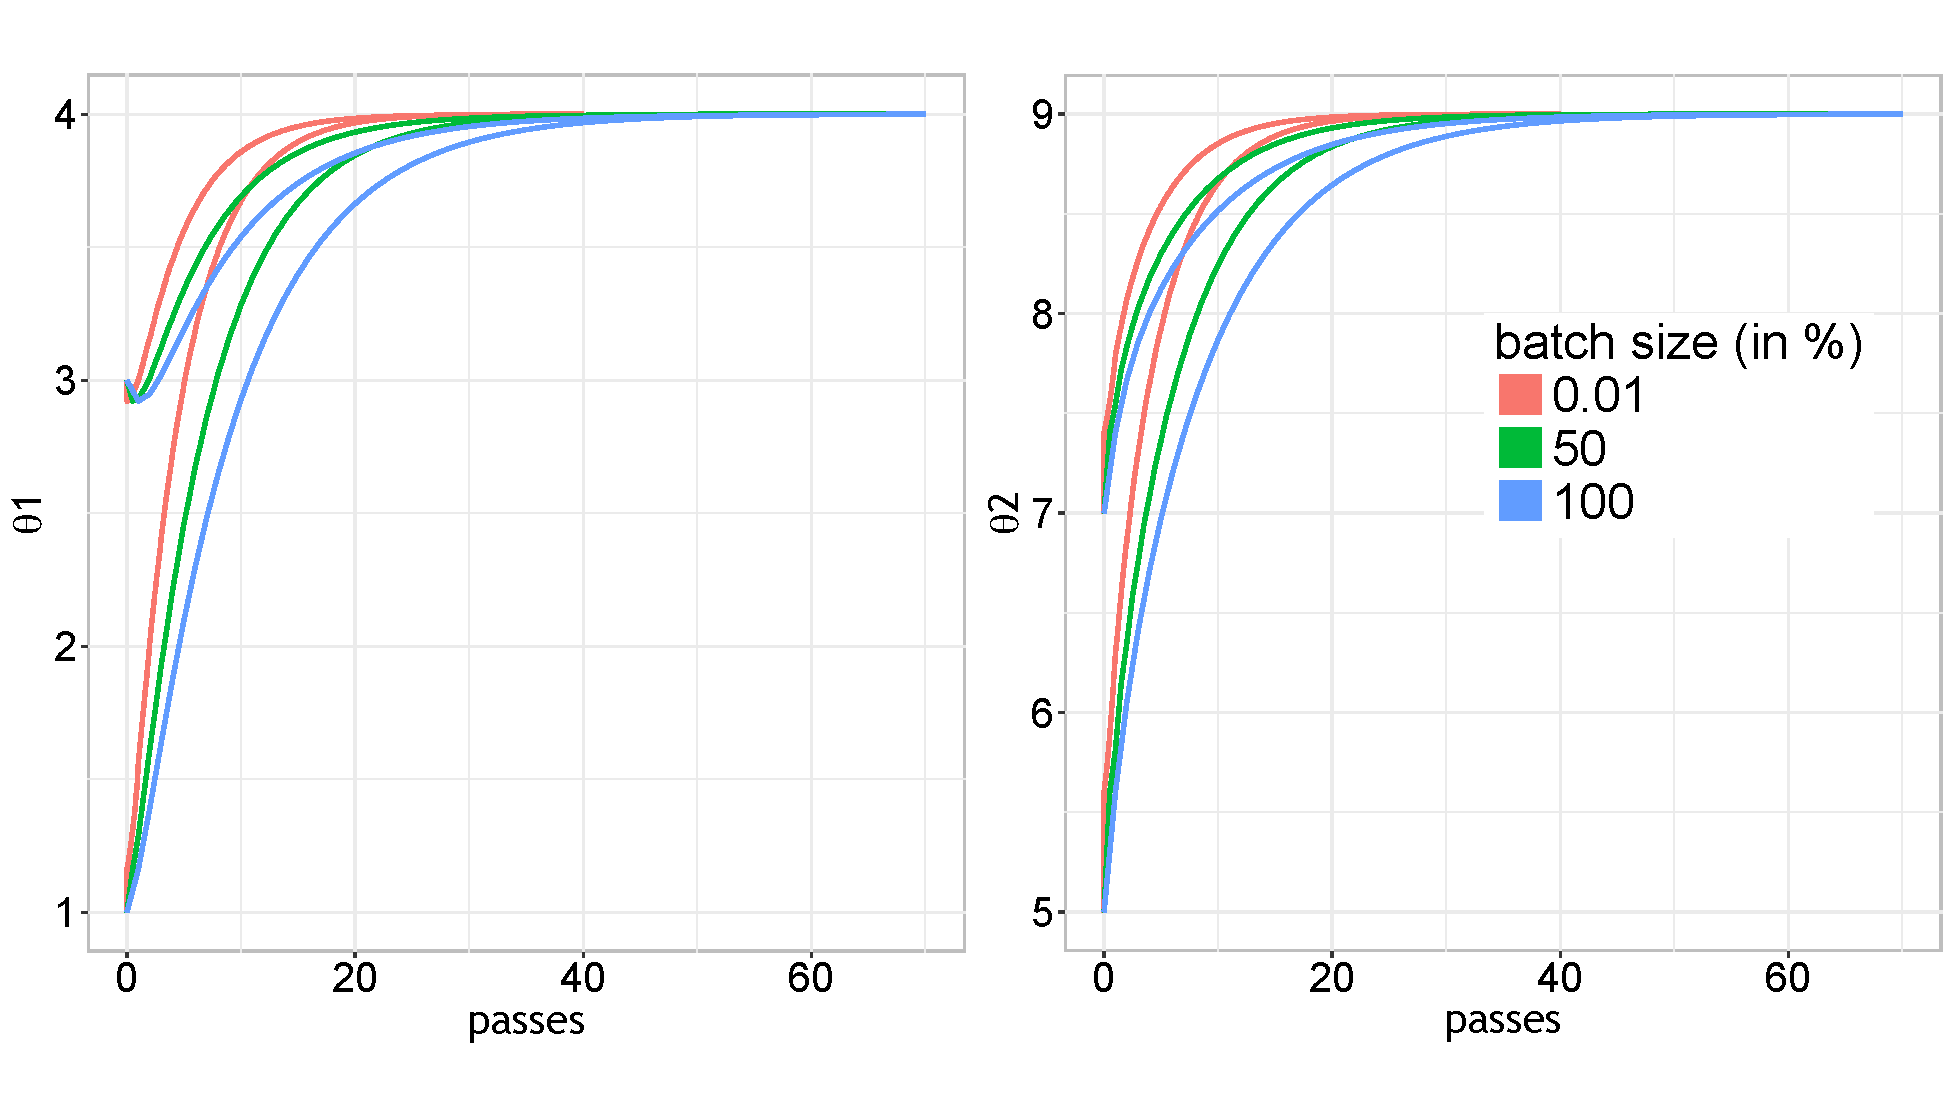
\includegraphics[scale = 0.35]{pics/iems.pdf}
\caption{Convergence of the vector of parameter estimates $\theta^k$ function of passes over the data.}
\label{iem_glm}
\end{center}
\end{figure}


\clearpage


\section{Proofs}\label{sec:proofs}

\subsection{Proof of Theorem 1}\label{proofs:IEM}
\subsubsection{Proof of (i)}
First, let us define for $\theta \in \Theta$
\begin{equation}\label{sumsurrogate}
 \bar{A}^k(\theta) \triangleq \sum_{i=1}^{N}{A^k_i(\theta)}\eqs,
\end{equation}
where for all $i \in \inter$, $A^{k}_{i}$ is defined in \eqref{Ai}. For any $k \geq 1$ and for all $\theta \in \Theta$ the following decomposition plays a key role:
\begin{equation}\label{deterquantity}
\bar{A}^k(\theta) = \bar{A}^{k-1}(\theta) + \sum_{i \in I_{k}}^{}{B_{i,\theta^{k-1}}(\theta)} - \sum_{i \in I_{k}}^{}{A^{k-1}_{i}(\theta)}.
\end{equation}
Since by construction $\bar{A}^k(\theta^k) \leq  \bar{A}^k(\theta^{k-1})$, we get:
\begin{align}\label{eq:decreasing}
\bar{A}^k(\theta^k) \leq \bar{A}^{k-1}(\theta^{k-1}) + \sum_{i \in I_{k}}^{}{B_{i,\theta^{k-1}}(\theta^{k-1})} - \sum_{i \in I_{k}}^{}{A^{k-1}_{i}(\theta^{k-1})}.
\end{align}
Since for $i \in I_k$, $B_{i,\theta^{k-1}}$ is a surrogate of $\loglike_i$ at $\theta^{k-1}$ we get that  $B_{i,\theta^{k-1}}(\theta^{k-1}) = \loglike_{i}(\theta^{k-1})$. On the other hand, for $i \in \inter$, $A^{k-1}_{i} \equiv B_{i,\theta^{\tau_{i,k-1}}}$ and $B_{i,\theta^{\tau_{i,k-1}}}$ is a surrogate of $\loglike_i$ at $\theta^{\tau_{i,k-1}}$, thus we obtain that $ \loglike_{i}(\theta^{k-1}) - A^{k-1}_{i}(\theta^{k-1}) \leq 0$. Plugging these two relations in \eqref{eq:decreasing}  we obtain:
\begin{align}
\bar{A}^k(\theta^k) & \leq \bar{A}^{k-1}(\theta^{k-1}) + \sum_{i \in I_{k}}^{}{\loglike_{i}(\theta^{k-1})} - \sum_{i \in I_{k}}^{}{A^{k-1}_{i}(\theta^{k-1})}\\
& \leq \bar{A}^{k-1}(\theta^{k-1})\eqs.
\end{align}
As a result, the sequence $\left(\bar{A}^k(\theta^k)\right)_{k\geq0}$ is monotonically decreasing.  Since, under assumption \cref{bounded}, this quantity is bounded from below with probability one, we obtain its almost sure convergence. Taking the expectations with respect to the sampling distributions of the previous inequalities implies the convergence of the (deterministic) sequence $\left(\E[\bar{A}^k(\theta^k)]\right)_{k\geq0}$. Let us denote for all $\theta \in \Theta$ and a subset $J \subset \inter$:
\begin{align}\label{batchnotation}
& \loglike_{J}(\theta) \triangleq \sum_{i \in J}^{}{\loglike_{i}(\theta)}\eqs,\\
& A^{k-1}_{J}(\theta) \triangleq \sum_{i \in J}^{}{A^{k-1}_{i}(\theta)}\eqs.
\end{align}
Inequality \eqref{eq:decreasing} gives :
\begin{align}
0 \leq \sum_{k=1}^{N}{A^{k-1}_{I_{k}}(\theta^{k-1}) - \loglike_{I_{k}}(\theta^{k-1})} \leq \sum_{k=1}^{N}{ \bar{A}^{k-1}(\theta^{k-1}) - \bar{A}^k(\theta^{k})} =  \bar{A}^{0}(\theta^{0}) - \bar{A}^n(\theta^{N})\eqs.
\end{align}
Consequently, the sum of positive terms $\left(\sum_{k=1}^{N}{A^{k-1}_{I_{k}}(\theta^{k-1}) - \loglike_{I_{k}}(\theta^{k-1})} \right)_{n \geq 1}$ converges almost surely and $\left(A^{k-1}_{I_{k}}(\theta^{k-1}) - \loglike_{I_{k}}(\theta^{k-1})\right)_{k\geq1}$ converges almost surely to zero.
The Beppo-Levi theorem and the Tower property of the conditional expectation imply:
\begin{align}\label{Mdeter1}
\mathsf{M} \triangleq \E \left[\sum_{k=0}^{\infty}{A^{k-1}_{I_{k}}(\theta^{k-1}) - \loglike_{I_{k}}(\theta^{k-1})}\right] & = \sum_{k=0}^{\infty}{\E \left[A^{k-1}_{I_{k}}(\theta^{k-1}) - \loglike_{I_{k}}(\theta^{k-1})\right]} \\
& = \sum_{k=0}^{\infty}{\E \left[\CPE{A^{k-1}_{I_{k}}(\theta^{k-1}) - \loglike_{I_{k}}(\theta^{k-1})}{\mathcal{F}_{k-1}} \right]}\eqs,
\end{align}
with 
\begin{align*}
& \CPE{\loglike_{I_{k}}(\theta^{k-1})}{\mathcal{F}_{k-1}} = \frac{p}{N} \loglike(\theta^{k-1}) \eqs,\\
& \CPE{[A^{k-1}_{I_{k}}(\theta^{k-1})}{\mathcal{F}_{k-1}} = \frac{p}{N} \sum_{i=1}^{N}{A^{k-1}_{i}(\theta^{k-1})} = \frac{p}{N}\bar{A}^{k-1}(\theta^{k-1}) \eqs,
\end{align*}
where $\mathcal{F}_{k-1} = \sigma(I_j, j \leq k-1)$ is the filtration generated by the sampling of the indices.
We thus obtain:
\begin{align}\label{Mdeter2}
\mathsf{M} =\frac{p}{N} \sum_{k=0}^{\infty}{\E \left[\bar{A}^{k-1}(\theta^{k-1}) - \loglike(\theta^{k-1})\right]} = \frac{p}{N} \E \left[\sum_{k=0}^{\infty}{\bar{A}^{k-1}(\theta^{k-1}) - \loglike(\theta^{k-1})}\right] < \infty \eqs.
\end{align}
This last equation shows that:
\begin{equation}\label{detergap}
    \lim \limits_{k \to \infty} \bar{A}^{k}(\theta^{k}) - \loglike(\theta^{k}) = 0 \quad \textrm{a.s.}
\end{equation}
which implies the almost sure convergence of $\left(\loglike(\theta^{k})\right)_{k\geq0}$.

\subsubsection{Proof of (ii)}
Let us define, for all $k \geq 0$, $\bar{h}_k$ as:
\begin{equation}\label{smoothH}
\bar{h}^k : \vartheta \to \sum_{i=1}^N{A^k_{i}(\vartheta) - \loglike_i(\vartheta)}\eqs.
\end{equation}
$\bar{h}^k$ is $L$-smooth with $L = \sum_{i=1}^N{L_i}$ since each of its component is $L_i$-smooth by definition of the surrogate functions. Using the particular parameter $\vartheta^k = \theta^k - \frac{1}{L}\nabla\bar{h}_k(\theta^k) $ we have the following classical inequality for smooth functions (cf. Lemma 1.2.3 in \citep{nesterov2007Gradient}):
\begin{align}\label{nest}
& 0 \leq \bar{h}^k(\vartheta^k) \leq \bar{h}^k(\theta^k) - \frac{1}{2L}\|\nabla\bar{h}^k(\theta^k)\|_2^2\\
\implies &  \|\nabla\bar{h}^k(\theta^k)\|_2^2 \leq 2L\bar{h}^k(\theta^k)\eqs.
\end{align}
Using \eqref{detergap}, we conclude that $\lim \limits_{k \to \infty}\|\nabla\bar{h}^k(\theta^k)\|_2 = 0$ a.s. Then, the decomposition of $\langle \nabla \loglike(\theta^k),\theta - \theta^k \rangle$ for any $\theta \in \Theta$ yields:

\begin{equation}
\langle \nabla \loglike(\theta^k),\theta - \theta^k \rangle = \langle \nabla \bar{A}^k(\theta^k), \theta - \theta^k \rangle - \langle \nabla\bar{h}^k(\theta^k),\theta - \theta^k \rangle\eqs.
\end{equation}
Note that $\theta^k$ is the result of the minimisation of the sum of surrogates $\bar{A}^k(\theta)$ on the constrained set $\Theta$, therefore  $\langle \nabla \bar{A}^k(\theta^k), \theta - \theta^k \rangle \geq 0$. Thus, we obtain, using the Cauchy-Schwarz inequality:
\begin{align}
\langle \nabla \loglike(\theta^k),\theta - \theta^k \rangle & \geq - \langle \nabla\bar{h}^k(\theta^k),\theta - \theta^k \rangle\\
& \geq - \|\nabla\bar{h}^k(\theta^k)\|_2 \|\theta - \theta^k\|_2 \eqs.
\end{align}
By minimising over $\Theta$ and taking the infimum limit on $k$, we get:
\begin{equation}
\liminf \limits_{k \to \infty}\inf \limits_{\theta \in \Theta} \frac{\langle \nabla \loglike(\theta^k),\theta - \theta^k \rangle}{\|\theta - \theta^k\|_2} \geq - \lim \limits_{k \to \infty}\|\nabla\bar{h}^k(\theta^k)\|_2 = 0 \eqs,
\end{equation}
which is the Asymptotic Stationary Point Condition  (ASPC).
\clearpage

\bibliographystyle{apalike}
\bibliography{ref}
\newpage
\printglossaries
\end{document} 